\documentclass[12pt,a4paper,titlepage]{article}
\usepackage{graphicx}
\usepackage[margin=1in]{geometry}
\usepackage{titling}

\usepackage{booktabs}
\usepackage[hidelinks]{hyperref}
\usepackage{float}


\usepackage{epstopdf}

\DeclareGraphicsExtensions{.png}
\DeclareGraphicsExtensions{.jpg}
%\DeclareGraphicsExtensions{.eps}

\begin{document}
\begin{titlepage}
	\begin{center}
		
		\begin{figure}[t]
			\centering
			
\includegraphics[width=350px]{UP_Logo.png}
		\end{figure}		
	
	
	\begin{flushright} 
		
		\textbf{\LARGE COS 301 Main Project}
		\newline \newline \newline
		\textbf{\LARGE Requirements and Design Specifications}
		\newline \newline \newline
 		\textbf{\LARGE ThinkTech}
		\newline \newline \newline
	\end{flushright}
		
		\vspace{1 cm}
		
		\LARGE{\textbf{Group Members: }}
		
		%\begin{minipage}{0.4\textwidth}

		\begin{flushright} \large
			Lelethu Zazaza 13028023\newline
			Goodness Adegbenro 13046412\newline
		\end{flushright}
		%\end{minipage}
		
	
		
		\textbf{Git repository link:\\}
		 \url{ https://github.com/COS301-ThinkTech}
		
		\vfill
		
		{\LARGE Version 0.1}
		\\
		{\large \today}		
		
		
	\end{center}
\end{titlepage}


\newpage
\tableofcontents


\pagebreak

\section{Background, Vision and Scope}
\subsection{Project background}
Without the correct or adequate number of resources, learning a new concept may turn out to be a daunting task. This is especially true for students who are studying a Computer Science course yet are not equipped with a practical or theoretical programming background. The motivation behind this project is to develop a tool that is intended to bridge the  gap between inexperience and practical application. The tool will provide the means to simulate program logic through flowcharts in a practical setting. 

\subsection{Project vision}

The aim of this project is to develop a flowchart and planning simulation tool that is simple and intuitive to use. Firstly, this will be accomplished by enhancing the visual nature of the application by making tools in certain contexts more prominent. Additionally, the application should provide informative and clear feedback to the user during the flowchart development phase. It is important that the look-and-feel of the application is uncluttered and uncomplicated so that the user feels at ease to experiment with the tools thereby enhancing the learning experience.

\subsection{Project scope}

The application is compromised of 2 units: flowchart development and flowchart simulation. An explanation of each unit will follow below.

\begin{itemize}
\item Flowchart development

The user is presented with a canvas upon which he can drop flowchart components to create a  complete flowchart.
The application will perform error checking on the constructed flowchart, so that (for example) multiple entry points into a program or certain flowchart components are not allowed. The applicatiom should also warn the user of instances of infinite loops or other  logical error possibilities. 

\item Flowchart simulation

The user should be able to run an error-free flowchart from start to finish. The system should allow for one-click execution of the entire program, as well as step-by-step execution. At all stages during execution, the currently executing component should be
highlighted, as well as the connection path being followed. The program's execution should
be very visually apparent and appealing. The output of the flowchart's execution should also
be apparent. 
\end{itemize}

The following components are specifically excluded from the scope of the project:

\begin{itemize}
\item No executable program code generation will be required for this project.
\item No complex design elements (such as user-defined component assemblies) are required.
Only the basic components of standard flowcharts are necessary.\\

\end{itemize}

\begin{figure}[H]
  \centering
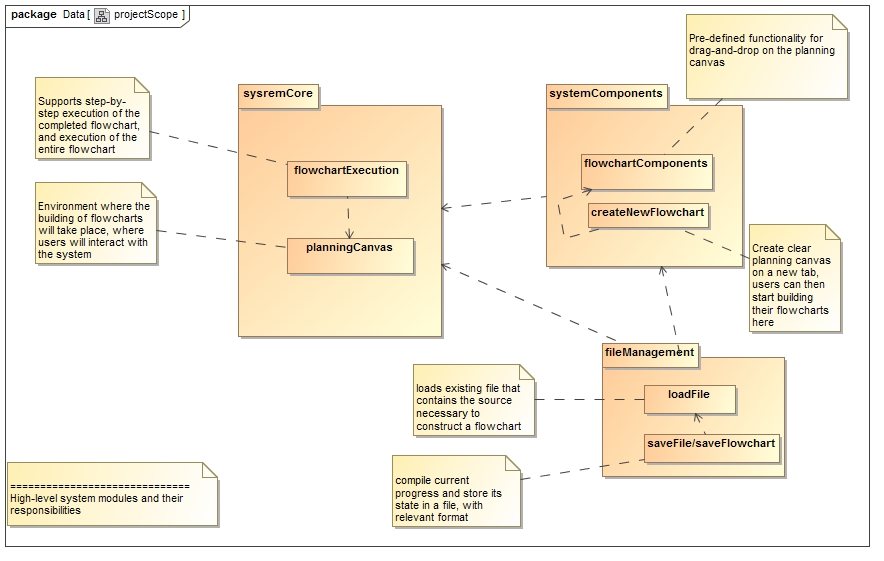
\includegraphics[width=500px]{projectScope.jpg}
\caption{High-level system modules and their responsibilities}
\end{figure}
% Include auxillary files here:  \input{file} 


\newpage	
\section{Use case prioritization}


\begin{table}[h!]   
    \label{tab:table1}
    \begin{tabular}{ccc}
      \toprule
      Critical & Important & Nice-To-Have\\
      \midrule	
%<<<<<<< HEAD
    
    %\end{tabular}  
%=======
	%\begin{tabular}{ccc}
      createFlowchartProject & addFlowchartComponent &  drag-and-drop components into bin\\
      deleteFlowchart & editFlowchartComponent & snap-to-grid development\\
       & deleteFlowchartComponent & predefined math functions\\
       & saveFlowchart & infinite-loop detection\\
       & loadFlowchart & logical-error detection\\
       & executeFlowchart & look-and-feel modification\\
      \bottomrule     
     \end{tabular}  
    \caption{Use case prioritization}
%>>>>>>> origin/master
\end{table}


\newpage
\section{Use cases}

\subsection{createFlowchartProject}
Creates an environment to enable users to start building flowcharts.\newline\newline
\textbf{Pre Condition:} Planning canvas must be blank.\newline\newline
\textbf{Post Condition:} New canvas with Start and Return component created.\newline
\textbf{Post Condition:} Flowchart Planning and Simulation tools ready for use.\newline

\begin{figure}[H]
  \centering
\includegraphics[width=500px]{createNewFlowchartProject.eps}
\caption{createFlowchartProject Use Case Diagram}
\end{figure}

\begin{figure}[H]
  \centering
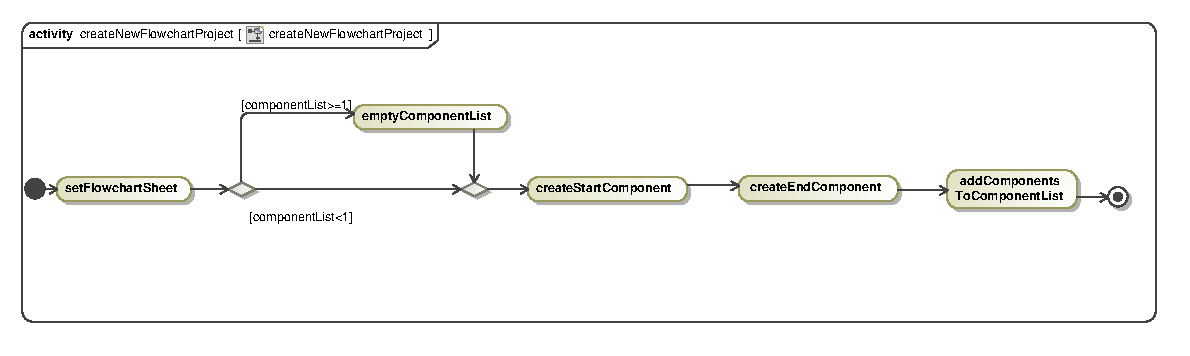
\includegraphics[width=500px]{createNewFlowchartProjectActivity.eps}
\caption{createFlowchartProject Activity Diagram}
\end{figure}

\newpage
\subsection{addFlowchartComponent}

Provides users with functionality to select the flowchart components they wish to place on the planning canvas.\newline\newline
\textbf{Pre Condition:} Canvas is available.\newline\newline
\textbf{Post Condition:} Component has been added to flowchart and appers on canvas with the necessary connections, if any.

\begin{figure}[H]
  \centering
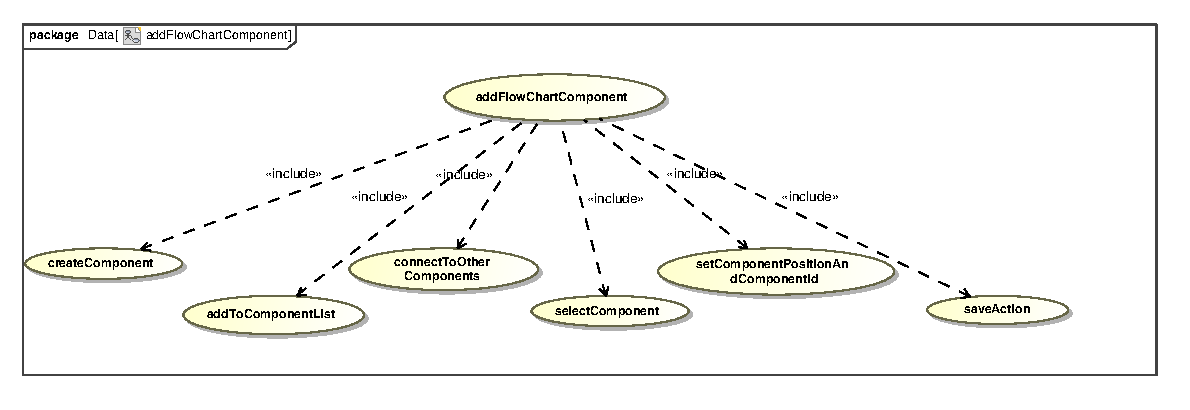
\includegraphics[width=500px]{addFlowChartComponent.eps}
\caption{addFlowchartComponent Use Case Diagram}
\end{figure}

\begin{figure}[H]
  \centering
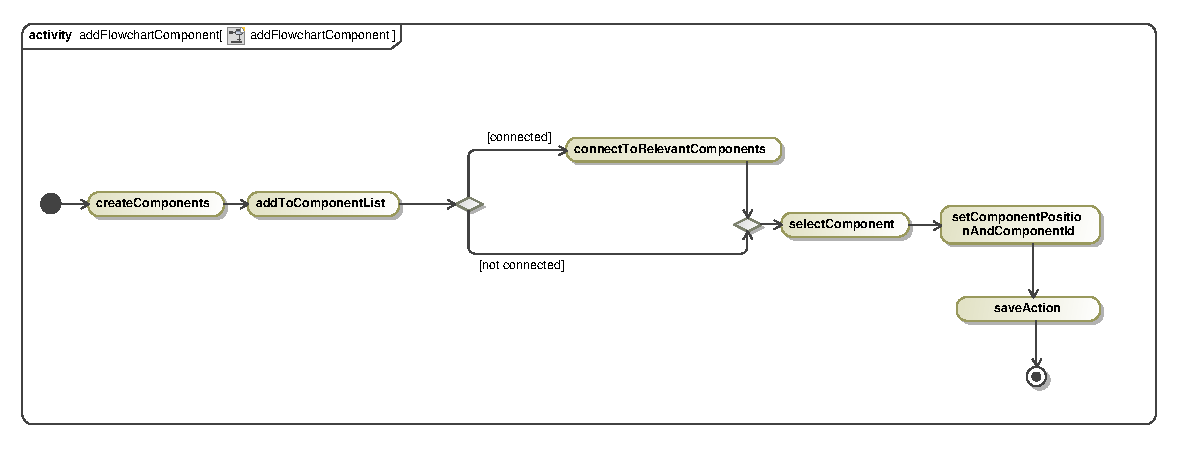
\includegraphics[width=500px]{addFlowchartComponentActivity.eps}
\caption{addFlowchartComponent Activity Diagram}
\end{figure}

\newpage
\subsection{editFlowchartComponent}

The editFlowchartComponent use case provides functionality for the user to edit each component of the flowchart on the canvas \newline\newline
\textbf{Pre Condition:} Canavas must exist.\newline
\textbf{Pre Condition:} Component must exist on active canvas.\newline\newline
\textbf{Post Condition:} Component has been edited.\newline
\textbf{Post Condition:} Edited component has been saved.

\begin{figure}[H]
  \centering
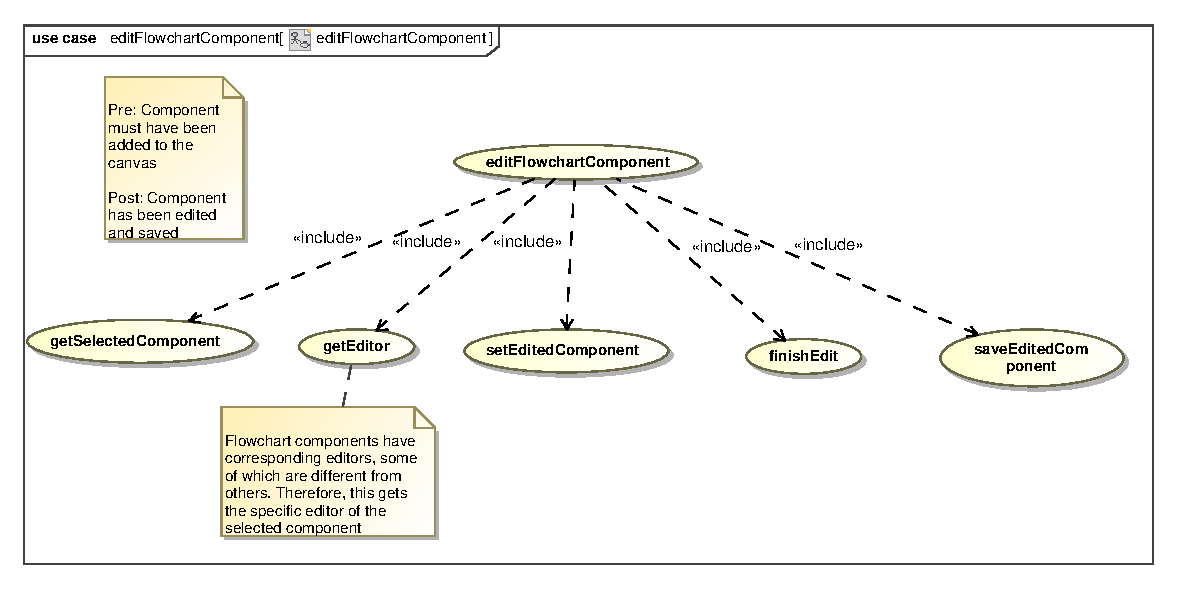
\includegraphics[width=500px]{editFlowchartComponent.eps}
\caption{editFlowchartComponent Use Case Diagram}
\end{figure}

\begin{figure}[H]
  \centering
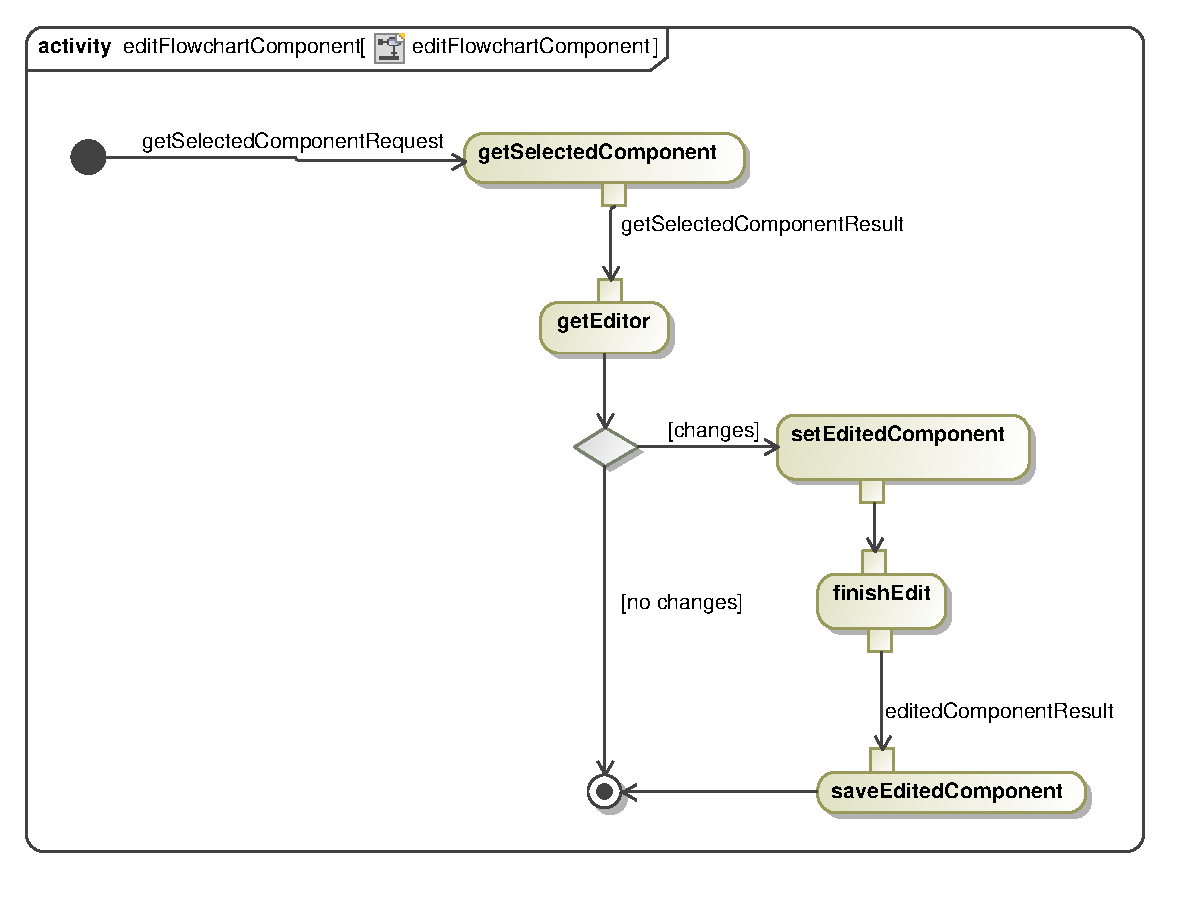
\includegraphics[width=300px]{editFlowchartComponentActivity.eps}
\caption{editFlowchartComponent Activity Diagram}
\end{figure}


\newpage
\subsection{deleteFlowchartComponent}
The deleteFlowchartComponent use case enables the functionality to delete individual components from the canvas.\newline\newline
\textbf{Pre Condition:} The canvas has to be available. \newline
\textbf{Pre Condition:} Component exists in the canvas space and is in the components list.\newline\newline
\textbf{Post Condition:} The canvas is clear of any components that were selected for removal.

\begin{figure}[H]
  \centering
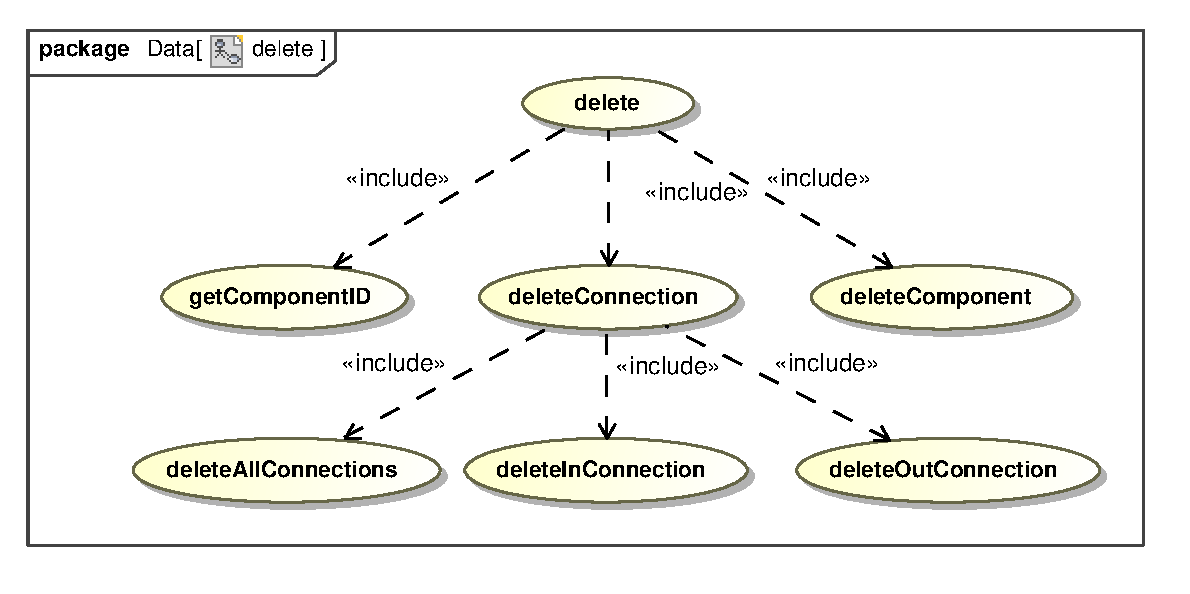
\includegraphics[width=500px]{delete.eps}
\caption{deleteFlowchartComponent Use Case Diagram}
\end{figure}

\begin{figure}[H]
  \centering
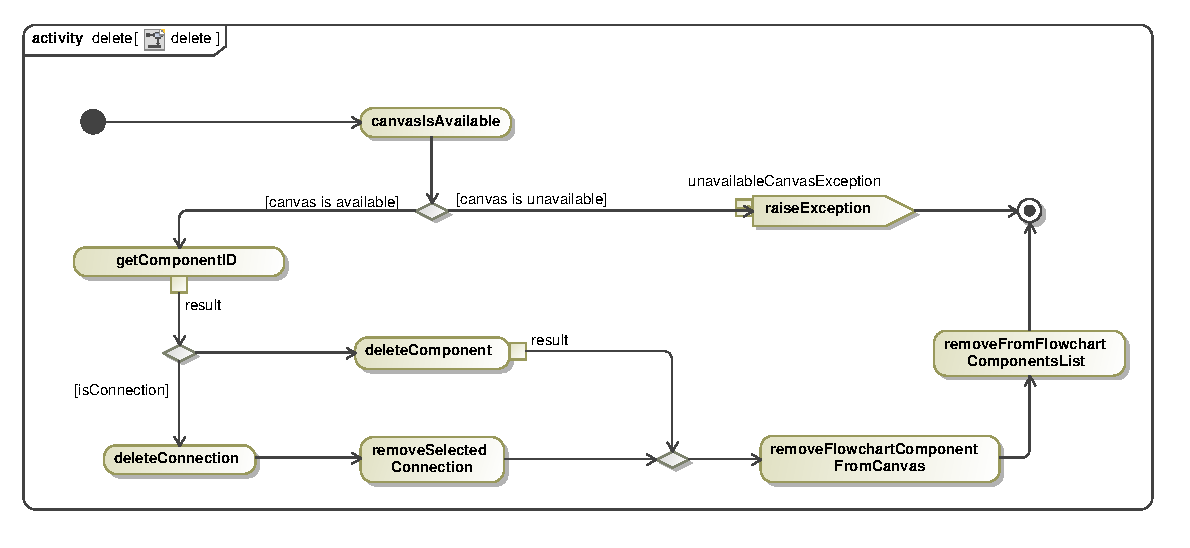
\includegraphics[width=500px]{deleteAct.eps}
\caption{deleteFlowchartComponent Activity Diagram}
\end{figure}

\newpage
\subsection{deleteFlowchart}
The deleteFlowchartProject use case serves the purpose of removing a flowchart project.\newline\newline
\textbf{Pre Condition:} Canvas exists.\newline
\textbf{Pre Condition:} Canvas is active.\newline
\textbf{Pre Condition:} The flowchart to be deleted must exist.\newline
\textbf{Pre Condition:} The flowchart to be deleted must be active.\newline\newline
\textbf{Post Condition:} The flowchart must be removed from the workspace and a new flowchart must then be created and made active on the workspace.

\begin{figure}[H]
  \centering
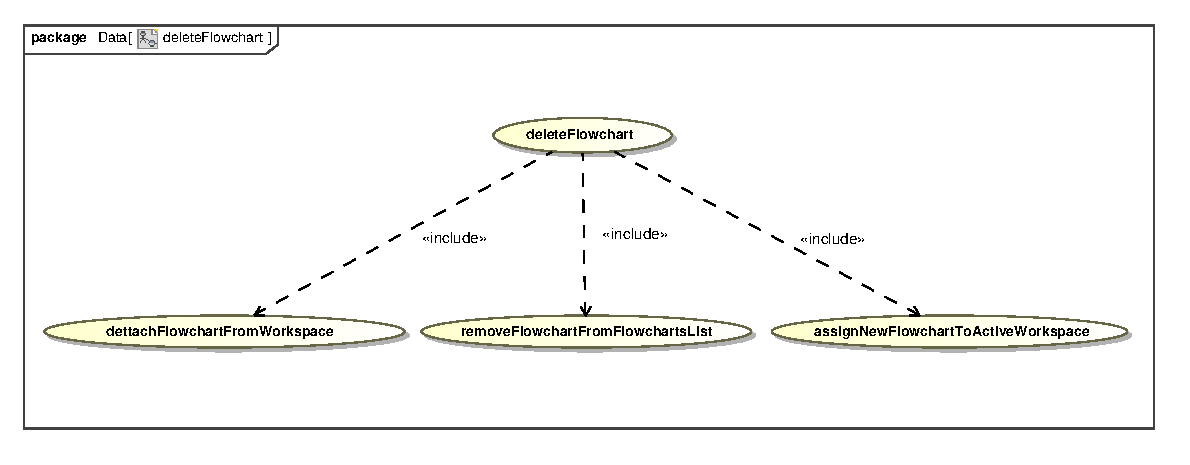
\includegraphics[width=500px]{deleteFlowchart.eps}
\caption{deleteFlowchart Use Case Diagram}
\end{figure}

\begin{figure}[H]
  \centering
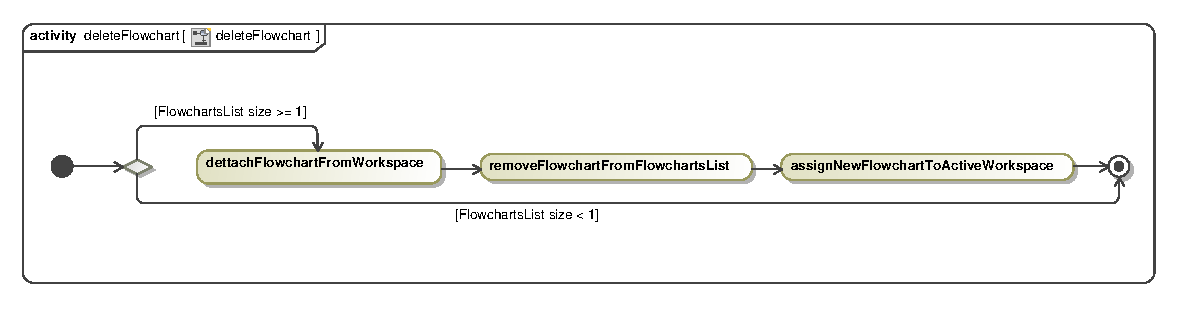
\includegraphics[width=500px]{deleteFlowchartActivity.eps}
\caption{deleteFlowchart Activity Diagram}
\end{figure}

\newpage
\subsection{saveFlowchart}
The saveFlowchart use case provides functionality for the user to save a flowchart.\newline\newline
\textbf{Pre Condition:} Canvas exists.\newline
\textbf{Pre Condition:} Canvas is active.\newline\newline
\textbf{Post Condition:} Flowchart has been saved to file.

\begin{figure}[H]
  \centering
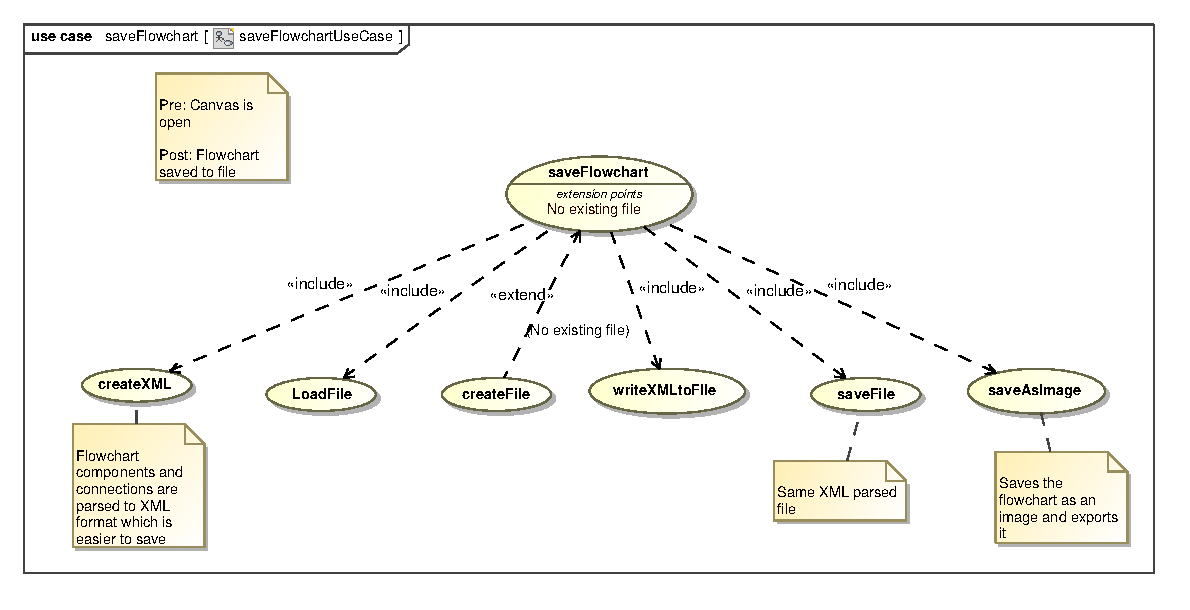
\includegraphics[width=500px]{saveFlowchartUseCase.eps}
\caption{saveFlowchart Use Case Diagram}
\end{figure}

\begin{figure}[H]
  \centering
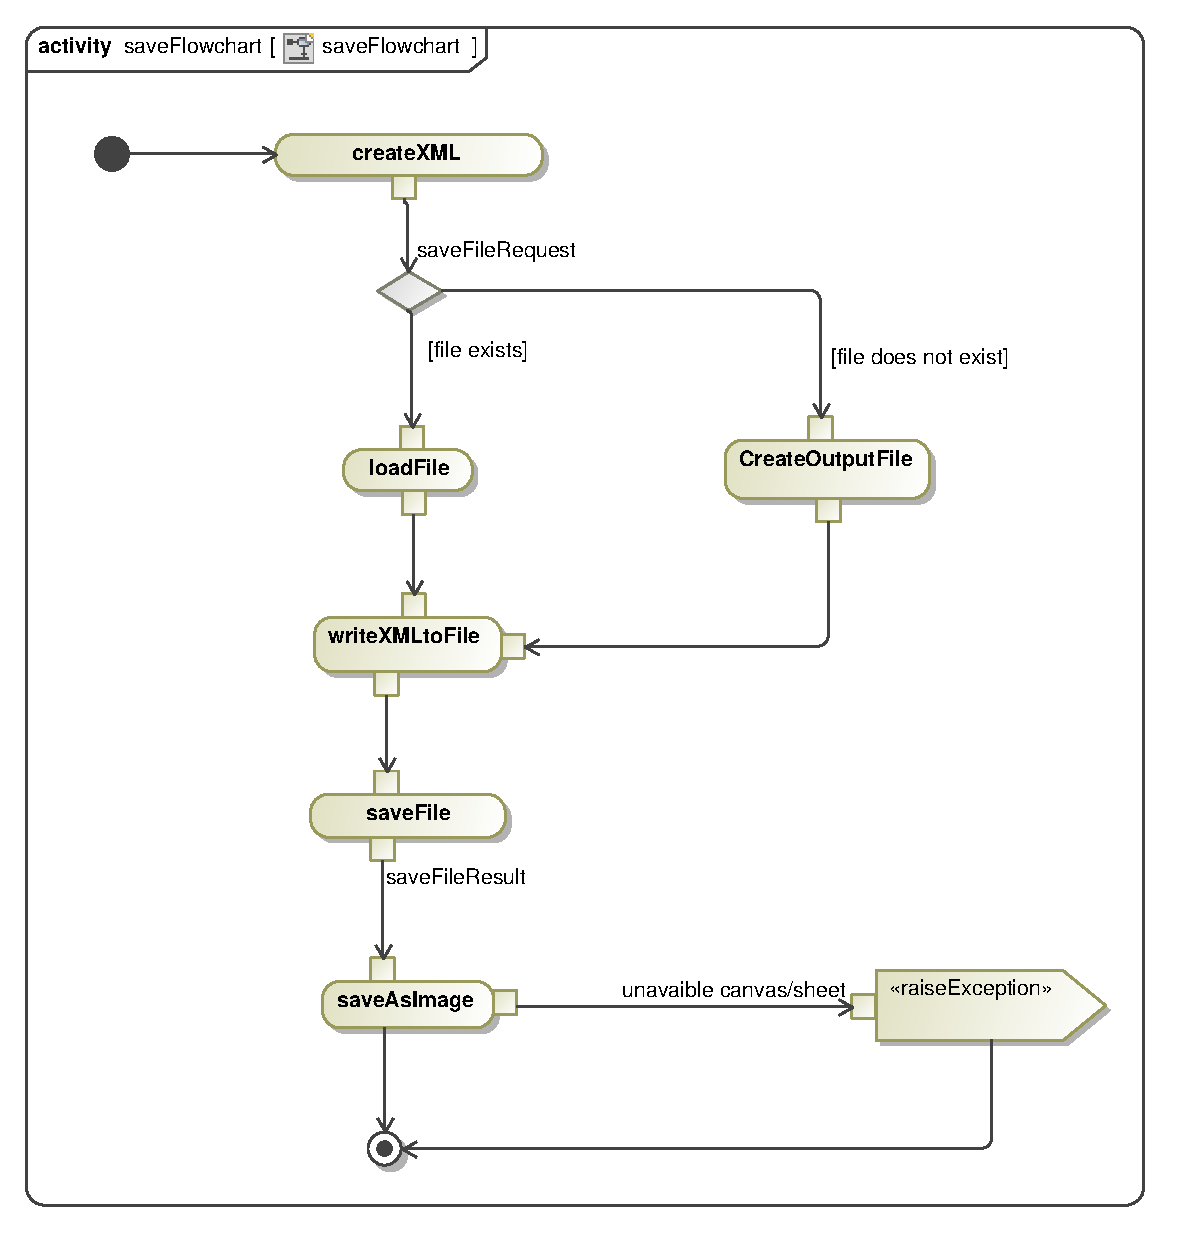
\includegraphics[height=250px, width=300px]{saveFlowchart.eps}
\caption{saveFlowchart Activity Diagram}
\end{figure}

\newpage
\subsection{loadFlowchart}
The loadFlowchart use case allows users load flowcharts from existing files. The file is editable and can be modified by the user.\newline\newline
\textbf{Pre Condition:} File with correct extension exists.\newline\newline
\textbf{Post Condition:} File contents have been converted and loaded on to the canvas.

\begin{figure}[H]
  \centering
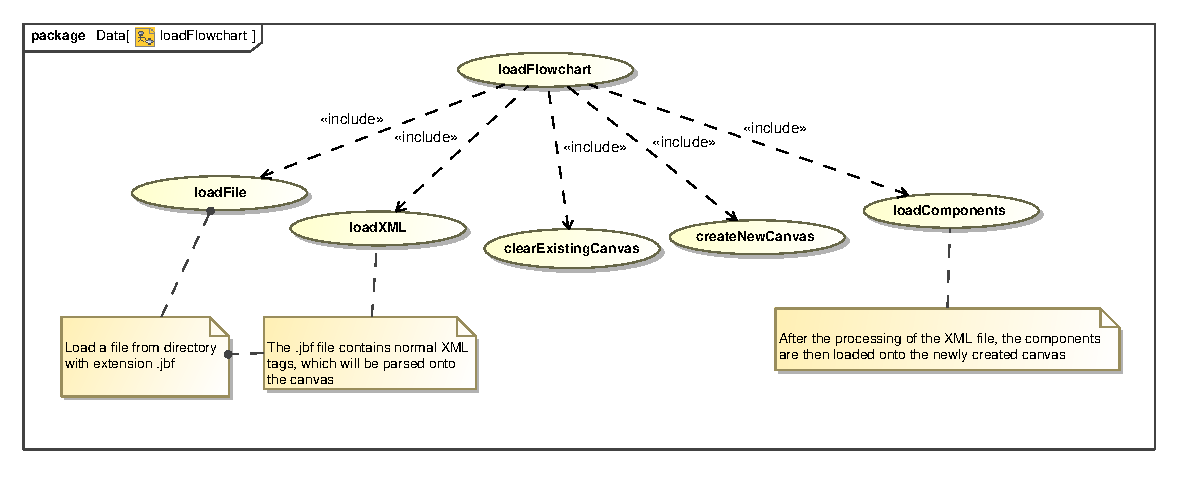
\includegraphics[width=500px]{loadFlowchart.eps}
\caption{loadFlowchart Use Case Diagram}
\end{figure}

\begin{figure}[H]
  \centering
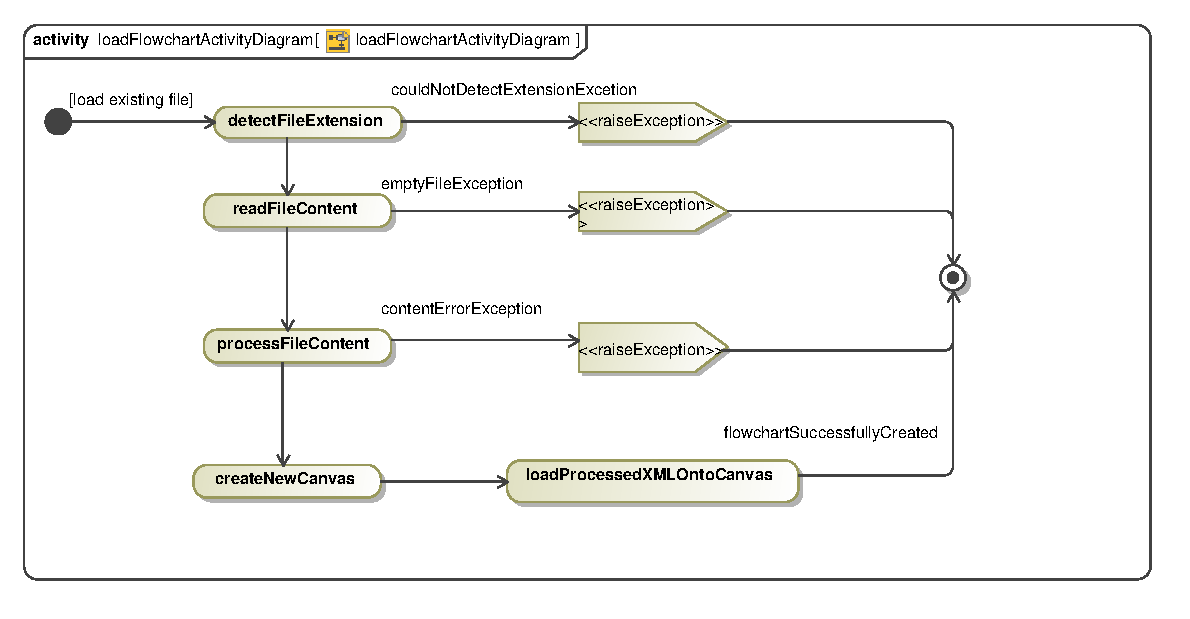
\includegraphics[width=500px]{loadFlowchartActivityDiagram.eps}
\caption{loadFlowchart Activity Diagram}
\end{figure}



\newpage
\subsection{executeFlowchart}
The executeFlowchart use case enables the functionality to execute the flowchart step-by-step or from start-to-end.\newline\newline
\textbf{Pre Condition:} Canvas has to be available.\newline\newline
\textbf{Post Condition:} Flowchart will return feedback of any errors, warnings or successful execution along with the results of any calculations.

\begin{figure}[H]
  \centering
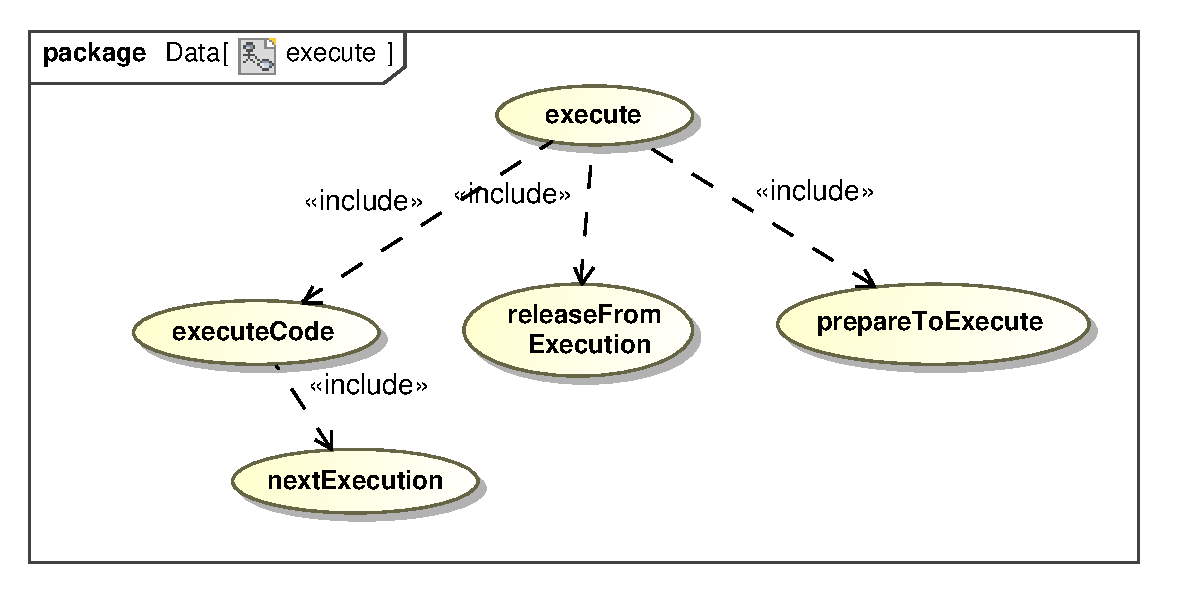
\includegraphics[width=500px]{execute.eps}
\caption{executeFlowchart Use Case Diagram}
\end{figure}

\begin{figure}[H]
  \centering
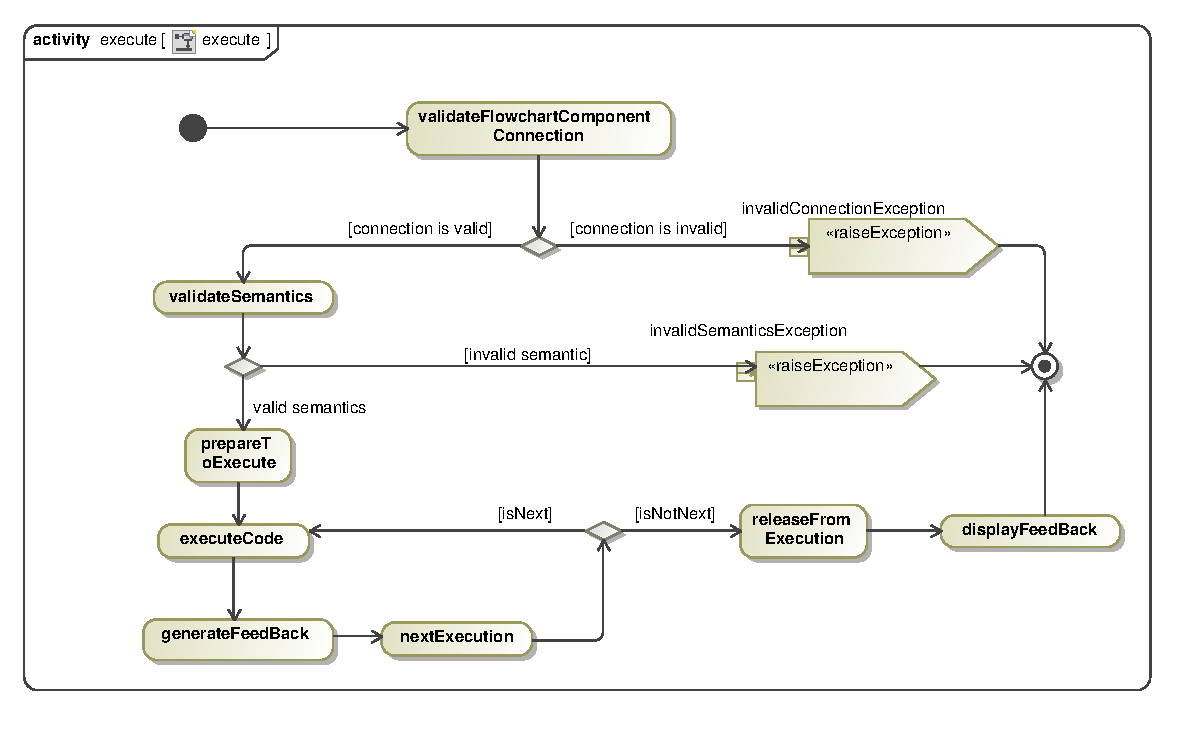
\includegraphics[width=385px]{executeAct.eps}
\caption{executeFlowchart Activity Diagram}
\end{figure}

\newpage
\section{The Domain Model - High-level}
\begin{figure}[H]
  \centering
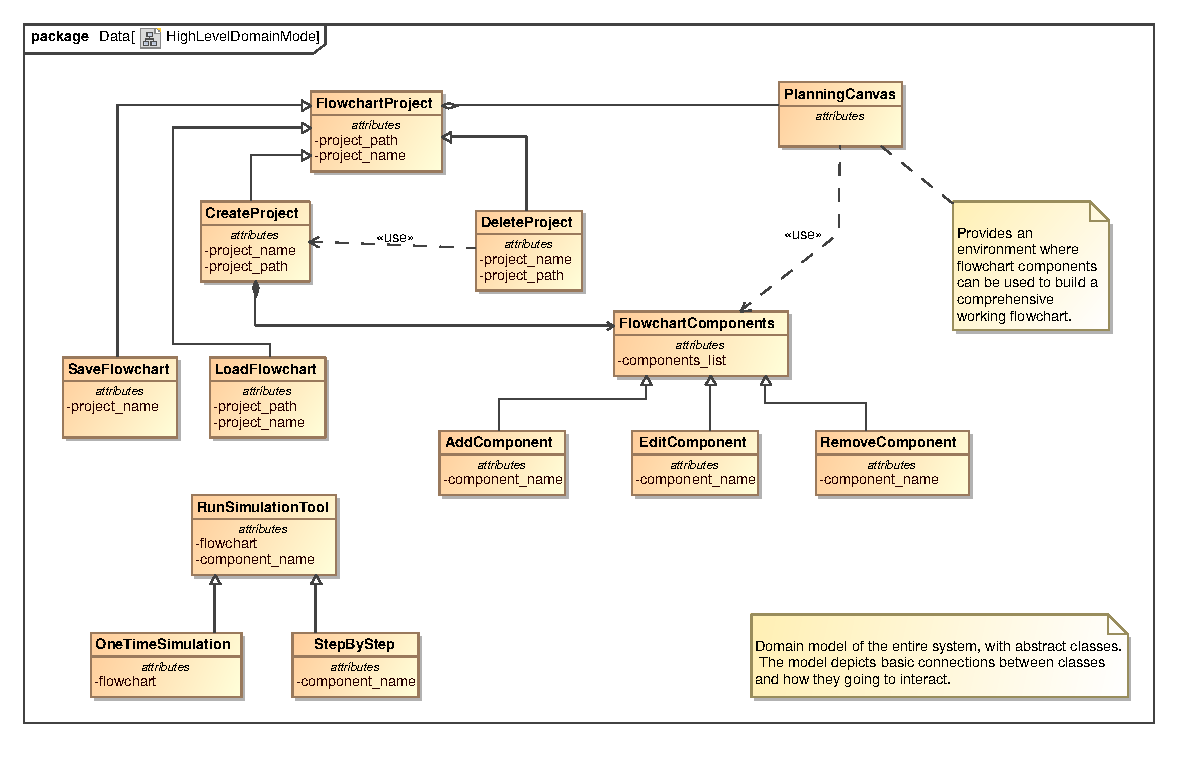
\includegraphics[width=500px]{HighLevelDomainModel.eps}
\caption{Domain Model Diagram}
\end{figure}

\newpage

%Short description of following contents
\section{Access and Integration Channels}
\subsection{Access Channels}
\subsubsection{Human access channels}

This application is accessible on a desktop computer running the Linux operating system, with a possibility of making the application accessible on a desktop computer running the Windows operating system.

\subsubsection{System access channels}
The system is not required to interface with any existing systems. It is only intended for execution on a desktop computer running the Linux operating system.

\subsection{Integration channels}
Since no other system interfaces with this system, no integration is required except of that of the internal modules.

\section{Architectural Responsibilities}

This system does not connect with any network, database or any other systems. Mostly it will depend on pure Java built-in functions.

\section{Quality Requirements}
%Quality Requirements to be added - Keagan & Maret
\begin{description}
  \item[Reliability:]
  	Any valid program expressed as a flowchart, without errors, is executable. In cases where errors are detected, sufficient feedback will be generated and provided to the user. A flowchart without any errors will generate output and feedback will also be provided.
 

  \item[Performance:]
  Performance is not a major concern. However, to ensure the system must provide feedback to the user during flowchart building and execution in a reasonable amount of time appropriate data structures and adequate design patterns will be used.

  \item[Maintainability:] 
  Since the whole system will be coded using Object-Oriented Programming (OOP), it will be much easy to update, extend and maintain the system. OOP allows the future development of the system.

  \item[Availability:]
  The application is available to all users, and can be executed on Windows and Linux machines.

  \item[Security:]
  This is a stand-alone application and it does not connect to any networks, so security is not a real concern.

  \item[Testability:]
  The GUI will provide a testing environment to the system, this will provide all the functionalities a standard and a complex flowchart can provide. When thorough GUI testing has been conducted, all detected malfunctions can be corrected.

  \item[Usability:]
  With the drag-and-drop functionality, the entire system will be very much easier to use; and also, pre-defined programming operations (eg. loops, conditional statements etc.) will be present. This is solely to enhance users to implement these operations without any standard programming language. Consequently the system will be independent of programming languages.
  

\end{description}
\section{Architecture Constraints}
%Architecture Constraints to be added - Johan & Latham
%Depending on which programming language best suits the interest of programmers, any language will be suitable. Preferably Java and C++. The system will resemble more or less the same programming styles used in Java and C++.

Because this system is built from an already existing system which was purely coded in Java, it is then highly recommended to implement the new system in Java. There are also numerous reasons for this, i.e., Java is a pure Object-oriented programming language which makes the code more readable and easier to read. This enhances maintainability.\newline

And also, the client specified that he needs an Object-oriented application, Java provides more precise Object-oriented features.

\section{Technologies}

As previously stated that the system that is being upgraded was coded in Java, this system as well will be coded in Java.
For testing, JUnit will be used. \newline

To save the current state of a flowchart, all the components of the flowchart will be processed into an XML file, to open the existing file, an XML will be parsed. So, XML will play a central role in managing the files.

% Add other things resemble programming technologies. e.g *** SWING *** ???



\end{document}




\newpage

\section{Architecture design}

\subsection{Overview}

The Model-View-Controller allows for dividing the application in three components, making the problem domain independent from the user interface.
A controller as the ability to send commands to the model to update the model's state (e.g., adding a component to the flowchart). It can also send commands to the associated view to change the view's presentation of the model (e.g. maximizing the flowchart window)
A model stores data that is retrieved by the controller and displayed in the view.
A view requests information from the model that it uses to generate an output representation to the user.


\subsection{Architectural tactics addressing quality requirements}

This section discusses the architectural tactics which are used to concretely address the quality requirements for the Flowchart and Simulation Tool application.

\subsubsection{Contracts based development}

Contracts allow the application to adhere to the following quality requirements:
Testability and maintainability.
The contracts will be enforced fo services  with pre and post-conditions which are assessed in unit tests, and data structure constraints enforced through data structure validation.

\subsubsection{Dependency Injection}

Dependency injection allows for the application to adhere to the following quality requirements:
Flexibility, deployability, testability.

\subsubsection{Minimize technology suite}

In order to improve maintainability the software architecture will minimize the number of programming languages  used.

\subsection{Architectural components}

This section discusses the architectural components and technologies used to address
the architectural responsibilities and the architectural tactics chosen to address the quality requirements

\subsubsection{Java}

Java is chosen as a single programming language used for the application in order to implement the tactic of minimizing the technology suite.  Using a single programming language reduces complexity and improves maintainability.

\subsubsection{JUnit}

JUnit will be used to achieve testability. With unit testing, we ensure that all module unit are precise and produce the expected results.

\subsection{Development architecture}

The development architecture is the architecture designed to support qualities in the development process itself. This
includes qualities like reliability.

\subsubsection{Version control}

The developer of the project make use of a git repository. Any new feature or bug should be developed in a new branch which is only merged into the trunk once the feature or passes its unit tests.

\subsection{IDE}

Each developer has the freedom to choose whichever IDE they prefer. 

\subsection{Builds}

To build the project artifacts Ant will be used. Ant is integrated with Netbeans IDE.

\subsection{Unit testing}

Unit testing will be done using JUnit which is a basic testing environment for Java applications.

\subsection{Integration testing}

This is a stand
\subsection{Bug tracking}

The projects will use GitHub's issue tracker for bug tracking.





	
\end{document}

